\documentclass[10pt]{article}
\input{style/coursHeadings}
\usepackage{algorithm}
\usepackage{algorithmic}


% Python sources
\usepackage{listings}
\usepackage{textcomp}
\usepackage{setspace}
%\usepackage{palatino}

%\usepackage{color}
\definecolor{Bleu}{rgb}{0.1,0.1,1.0}
\definecolor{Noir}{rgb}{0,0,0}
\definecolor{Grau}{rgb}{0.5,0.5,0.5}
\definecolor{DunkelGrau}{rgb}{0.15,0.15,0.15}
\definecolor{Hellbraun}{rgb}{0.5,0.25,0.0}
\definecolor{Magenta}{rgb}{1.0,0.0,1.0}
\definecolor{Gris}{gray}{0.5}
\definecolor{Vert}{rgb}{0,0.5,0}
\definecolor{SourceHintergrund}{rgb}{1,1.0,0.95}

%
\renewcommand{\lstlistlistingname}{Listings}
\renewcommand{\lstlistingname}{Listing}

\lstnewenvironment{python}[1][]{
\lstset{
language=python,
basicstyle=\ttfamily\footnotesize\setstretch{1}, 	
stringstyle=\color{red}, 
showstringspaces=false, 
alsoletter={1234567890},
otherkeywords={\ , \}, \{},
keywordstyle=\color{blue},
emph={access,and,break,class,continue,def,del,elif ,else,
except,exec,finally,for,from,global,if,import,in,i s,
lambda,not,or,pass,print,raise,return,try,while},
emphstyle=\color{black}\bfseries,
emph={[2]True, False, None, self},
emphstyle=[2]\color{green},
emph={[3]from, import, as},
emphstyle=[3]\color{blue},
upquote=true,
morecomment=[s]{"""}{"""},
commentstyle=\color{Hellbraun}\slshape, 
%emph={[4]1, 2, 3, 4, 5, 6, 7, 8, 9, 0},
emphstyle=[4]\color{blue},
literate=*{:}{{\textcolor{blue}:}}{1}
{=}{{\textcolor{blue}=}}{1}
{-}{{\textcolor{blue}-}}{1}
{+}{{\textcolor{blue}+}}{1}
{*}{{\textcolor{blue}*}}{1}
{!}{{\textcolor{blue}!}}{1}
{(}{{\textcolor{blue}(}}{1}
{)}{{\textcolor{blue})}}{1}
{[}{{\textcolor{blue}[}}{1}
{]}{{\textcolor{blue}]}}{1}
{<}{{\textcolor{blue}<}}{1}
{>}{{\textcolor{blue}>}}{1},
%framexleftmargin=1mm, framextopmargin=1mm, frame=shadowbox, rulesepcolor=\color{blue},#1
backgroundcolor=\color{SourceHintergrund}, 
framexleftmargin=1mm, framexrightmargin=1mm, framextopmargin=1mm, frame=single, framerule=1pt, rulecolor=\color{black},#1
}}{}
%%%%%%%%%%%%
% Définition des vecteurs 
%%%%%%%%%%%%
\newcommand{\vect}[1]{\overrightarrow{#1}}
\newcommand{\axe}[2]{\left(#1,\vect{#2}\right)}
\newcommand{\couple}[2]{\left(#1,\vect{#2}\right)}
\newcommand{\angl}[2]{\left(\vect{#1},\vect{#2}\right)}

\newcommand{\rep}[1]{\mathcal{R}_{#1}}
\newcommand{\quadruplet}[4]{\left(#1;#2,#3,#4 \right)}
\newcommand{\repere}[4]{\left(#1;\vect{#2},\vect{#3},\vect{#4} \right)}
\newcommand{\base}[3]{\left(\vect{#1},\vect{#2},\vect{#3} \right)}


\newcommand{\vx}[1]{\vect{x_{#1}}}
\newcommand{\vy}[1]{\vect{y_{#1}}}
\newcommand{\vz}[1]{\vect{z_{#1}}}

\newcommand{\norm}[1]{\ensuremath{\left\Vert {#1}\right\Vert}}
\newcommand{\Ker}{\mathop{\mathrm{Ker}}\nolimits}

% d droit pour le calcul différentiel
\newcommand{\dd}{\text{d}}

\newcommand{\inertie}[2]{I_{#1}\left( #2\right)}
\newcommand{\matinertie}[7]{
\begin{pmatrix}
#1 & #6 & #5 \\
#6 & #2 & #4 \\
#5 & #4 & #3 \\
\end{pmatrix}_{#7}}
%%%%%%%%%%%%
% Définition des torseurs 
%%%%%%%%%%%%

\newcommand{\ec}[2]{%
\mathcal{E}_c\left(#1/#2\right)}

\newcommand{\pext}[3]{%
\mathcal{P}\left(#1\rightarrow#2/#3\right)}

\newcommand{\pint}[3]{%
\mathcal{P}\left(#1 \stackrel{\text{#3}}{\leftrightarrow} #2\right)}


 \newcommand{\torseur}[1]{%
\left\{{#1}\right\}
}

\newcommand{\torseurcin}[3]{%
\left\{\mathcal{#1} \left(#2/#3 \right) \right\}
}

\newcommand{\torseurci}[2]{%
\left\{\sigma \left(#1/#2 \right) \right\}
}
\newcommand{\torseurdyn}[2]{%
\left\{\mathcal{D} \left(#1/#2 \right) \right\}
}


\newcommand{\torseurstat}[3]{%
\left\{\mathcal{#1} \left(#2\rightarrow #3 \right) \right\}
}


 \newcommand{\torseurc}[8]{%
%\left\{#1 \right\}=
\left\{
{#1}
\right\}
 = 
\left\{%
\begin{array}{cc}%
{#2} & {#5}\\%
{#3} & {#6}\\%
{#4} & {#7}\\%
\end{array}%
\right\}_{#8}%
}

 \newcommand{\torseurcol}[7]{
\left\{%
\begin{array}{cc}%
{#1} & {#4}\\%
{#2} & {#5}\\%
{#3} & {#6}\\%
\end{array}%
\right\}_{#7}%
}

 \newcommand{\torseurl}[3]{%
%\left\{\mathcal{#1}\right\}_{#2}=%
\left\{%
\begin{array}{l}%
{#1} \\%
{#2} %
\end{array}%
\right\}_{#3}%
}

% Vecteur vitesse
 \newcommand{\vectv}[3]{%
\vect{V\left( {#1} \in {#2}/{#3}\right)}
}

% Vecteur force
\newcommand{\vectf}[2]{%
\vect{R\left( {#1} \rightarrow {#2}\right)}
}

% Vecteur moment stat
\newcommand{\vectm}[3]{%
\vect{\mathcal{M}\left( {#1}, {#2} \rightarrow {#3}\right)}
}




% Vecteur résultante cin
\newcommand{\vectrc}[2]{%
\vect{R_c \left( {#1}/ {#2}\right)}
}
% Vecteur moment cin
\newcommand{\vectmc}[3]{%
\vect{\sigma \left( {#1}, {#2} /{#3}\right)}
}


% Vecteur résultante dyn
\newcommand{\vectrd}[2]{%
\vect{R_d \left( {#1}/ {#2}\right)}
}
% Vecteur moment dyn
\newcommand{\vectmd}[3]{%
\vect{\delta \left( {#1}, {#2} /{#3}\right)}
}

% Vecteur accélération
 \newcommand{\vectg}[3]{%
\vect{\Gamma \left( {#1} \in {#2}/{#3}\right)}
}

% Vecteur omega
 \newcommand{\vecto}[2]{%
\vect{\Omega\left( {#1}/{#2}\right)}
}
% }$$\left\{\mathcal{#1} \right\}_{#2} =%
% \left\{%
% \begin{array}{c}%
%  #3 \\%
%  #4 %
% \end{array}%
% \right\}_{#5}}

\newcommand{\N}{\mathbb{N}}
\newcommand{\Z}{\mathbb{Z}}
\newcommand{\R}{\mathbb{R}}
\newcommand{\C}{\mathbb{C}}
\newcommand{\K}{\mathbb{K}}

\newcommand{\cA}{\mathscr{A}}
\newcommand{\cM}{\mathscr{M}}
\newcommand{\cL}{\mathscr{L}}
\newcommand{\cS}{\mathscr{S}}

\newcommand{\python}{\texttt{Python}}

\newcommand{\z}[1]{\Z_{#1}}
\newcommand{\ztimes}[1]{\Z_{#1}^{\times}}
\newcommand{\ii}[1]{[\![#1[\![}
\newcommand{\iif}[1]{[\![#1]\!]}
\newcommand{\llbr}{\ensuremath{\llbracket}}
\newcommand{\rrbr}{\ensuremath{\rrbracket}}
%\newcommand{\p}[1]{\left(#1\right)}
\newcommand{\ens}[1]{\left\{ #1 \right\}}
\newcommand{\croch}[1]{\left[ #1 \right]}
%\newcommand{\of}[1]{\lstinline{#1}}
% \newcommand{\py}[2]{%
%   \begin{tabular}{|l}
%     \lstinline+>>>+\textbf{\of{#1}}\\
%     \of{#2}
%   \end{tabular}\par{}
% }
\newcommand{\floor}[1]{\left\lfloor#1\right\rfloor}
\newcommand{\ceil}[1]{\left\lceil#1\right\rceil}
\newcommand{\abs}[1]{\left|#1\right|}


% Binaire, octal, hexa
\newcommand{\hex}[1]{\underline{\text{\texttt{#1}}}_{16}}
\newcommand{\oct}[1]{\underline{\text{\texttt{#1}}}_{8}}
\newcommand{\bin}[1]{\underline{\text{\texttt{#1}}}_{2}}
\DeclareMathOperator{\mmod}{\texttt{\%}}


% Fonctions et systèmes
\newcommand{\fct}[5][t]{%
  \begin{array}[#1]{rcl}
    #2 & \rightarrow & #3\\
    #4 & \mapsto     & #5\\
  \end{array}
}
\newcommand{\fonction}[5]{#1 : \left\{\begin{array}{rcl} #2& \longrightarrow &#3 \\ #4 &\longmapsto & #5\end{array}\right.}
\newenvironment{systeme}{\left\{ \begin{array}{rcl}}{\end{array}\right.}

% Matrices
\newcommand{\mat}[1]{
  \begin{pmatrix}
    #1
  \end{pmatrix}
}
\newcommand{\inv}{\ensuremath{^{-1}}}
\newcommand{\bpm}{\begin{pmatrix}}
\newcommand{\epm}{\end{pmatrix}}


% bases de données
\newcommand{\relat}[1]{\textsc{#1}}
\newcommand{\attr}[1]{\emph{#1}}
\newcommand{\prim}[1]{\uline{#1}}
\newcommand{\foreign}[1]{\#\textsl{#1}}


% Bases de données

\newcommand{\att}{\ensuremath{\mathbf{att}}}
\newcommand{\dom}{\ensuremath{\mathbf{dom}}}
\newcommand{\sort}{\ensuremath{\mathbf{sort}}}
\newcommand{\relname}{\ensuremath{\mathbf{relname}}}
\newcommand{\var}{\ensuremath{\mathbf{var}}}
\newcommand{\FILM}{\ensuremath{\mathtt{FILM}}}
\newcommand{\JOUE}{\ensuremath{\mathtt{JOUE}}}
\newcommand{\PERSONNE}{\ensuremath{\mathtt{PERSONNE}}}
\newcommand{\PERSONNAGE}{\ensuremath{\mathtt{PERSONNAGE}}}

\newcommand{\ttid}{\ensuremath{\mathtt{id}}}
\newcommand{\tttitre}{\ensuremath{\mathtt{titre}}}
\newcommand{\ttdate}{\ensuremath{\mathtt{date}}}
\newcommand{\ttidr}{\ensuremath{\mathtt{idrealisateur}}}
\newcommand{\ttdatenais}{\ensuremath{\mathtt{datenaissance}}}
\newcommand{\ttnom}{\ensuremath{\mathtt{nom}}}
\newcommand{\ttprenom}{\ensuremath{\mathtt{prenom}}}
\newcommand{\ttidacteur}{\ensuremath{\mathtt{idacteur}}}
\newcommand{\ttidfilm}{\ensuremath{\mathtt{idfilm}}}
\newcommand{\ttidpersonnage}{\ensuremath{\mathtt{idpersonnage}}}

\newcommand{\fv}{\mathrm{libre}}
\newcommand{\sem}[1]{[\![ #1 ]\!]}

\input{style/macros_Titres}
\input{style/macros_Frames}


%Si le boolen xp est vrai : compilation pour xabi
%Sinon compilation Damien
\newboolean{xp}
\setboolean{xp}{true}

\newboolean{prof}
\setboolean{prof}{true}

\usepackage[%
    pdftitle={Problèmes stationnaires},
    pdfauthor={Xavier Pessoles},
    colorlinks=true,
    linkcolor=blue,
    citecolor=magenta]{hyperref}


\def\discipline{Informatique}
\def\xxtitre{\ifthenelse{\boolean{xp}}{
CI 3 : Ingénierie Numérique \& Simulation}{
Chapitre  -- }}

\def\xxsoustitre{\ifthenelse{\boolean{xp}}{
Chapitre 3 -- Résolution des équation différentielles}{
Partie  -- }}

\def\xxauteur{\ifthenelse{\boolean{xp}}{
Xavier \textsc{Pessoles}}{
Damien \textsc{Iceta} \\ Xavier \textsc{Pessoles}}}

\def\xxpied{\ifthenelse{\boolean{xp}}{
CI 3 : Ingénierie Numérique \& Simulation\\
Ch. 3 : Résolution des équations différentielles -- Cours}{
\xxtitre}}

\def\xxcathegorie{\ifthenelse{\boolean{xp}}{
2013 -- 2014 \\
Xavier \textsc{Pessoles}}{
Informatique - Cours}}





%---------------------------------------------------------------------------


\begin{document}

\ifthenelse{\boolean{xp}}{\usepackage[%
    pdftitle={Représentation des nombres},
    pdfauthor={Xavier Pessoles},
    colorlinks=true,
    linkcolor=blue,
    citecolor=magenta]{hyperref}

\usepackage{pifont}
%\usepackage{lastpage}

% \makeatletter \let\ps@plain\ps@empty \makeatother
%% DEBUT DU DOCUMENT
%% =================
\sloppy
\hyphenpenalty 10000


\colorlet{shadecolor}{orange!15}

\newtheorem{theorem}{Theorem}


\begin{document}


%\newboolean{prof}
%\setboolean{prof}{true}
% \makeatletter \let\ps@plain\ps@empty \makeatother
%% DEBUT DU DOCUMENT
%% =================




%------------- En tetes et Pieds de Pages ------------


\pagestyle{fancy}
\ifthenelse{\boolean{xp}}{%
\renewcommand{\headrulewidth}{0pt}}{%
\renewcommand{\headrulewidth}{0.2pt}} %pour mettre le trait en haut
%\renewcommand{\headrulewidth}{0.2pt}

\fancyhead{}
\fancyhead[L]{%
\noindent\begin{minipage}[c]{2.6cm}%
\includegraphics[width=2cm]{png/logo_ptsi.png}%
\end{minipage}}


\fancyhead[C]{\rule{12cm}{.5pt}}



\fancyhead[R]{%
\noindent\begin{minipage}[c]{3cm}
\begin{flushright}
\footnotesize{\textit{\textsf{Informatique}}}%
\end{flushright}
\end{minipage}
}



\fancyhead[C]{\rule{12cm}{.5pt}}

\renewcommand{\footrulewidth}{0.2pt}

\fancyfoot[C]{\footnotesize{\bfseries \thepage}}
\fancyfoot[L]{%
\begin{minipage}[c]{.2\linewidth}
\noindent\footnotesize{{\xxauteur}}
\end{minipage}
\ifthenelse{\boolean{xp}}{}{%
\begin{minipage}[c]{.15\linewidth}
\includegraphics[width=2cm]{png/logoCC.png}
\end{minipage}}
}

\ifthenelse{\boolean{prof}}{%
\fancyfoot[R]{\footnotesize{\xxpied}}}

\begin{center}
 \huge\textsc{\xxtitre}
\end{center}

\begin{center}
 \LARGE\textsc{\xxsoustitre}
\end{center}

\vspace{.5cm}
}{\input{style/enteteDI}}

\begin{minipage}[c]{.2\linewidth}
\begin{center}
%\includegraphics[width=.95\textwidth]{images/swing}
\end{center}
\end{minipage}\hfill
\begin{minipage}[c]{.33\linewidth}
\begin{center}
%\includegraphics[width=.9\textwidth]{images/situation}
\end{center}
\end{minipage}\hfill
\begin{minipage}[c]{.45\linewidth}
\begin{center}
%\includegraphics[width=.95\textwidth]{images/tir_alpha}
\end{center}
\end{minipage}
\vspace{.5cm}

\begin{savoir}
Problème dynamique à une dimension,  linéaire ou non, conduisant à la résolution approchée d’une équation différentielle ordinaire par la méthode d’Euler.
\end{savoir}



\setlength{\parskip}{0ex plus 0.2ex minus 0ex}
 \renewcommand{\contentsname}{}
 \renewcommand{\baselinestretch}{1}

\tableofcontents

 \renewcommand{\baselinestretch}{1.2}
\setlength{\parskip}{2ex plus 0.5ex minus 0.2ex}





\section{Présentation}

\subsection{Contexte}

\begin{defi}
\textbf{Équation différentielle ordinaire -- EDO}

Soit $I$ un intervalle compact (\textit{ie.} fermé et borné) non vide. $I\in\mathbb{R}$. 

Soit $f$ une application continue telle que : 
$$
(t,x)\in I \times \mathbb{R}^m \rightarrow f(t,x)\in \mathbb{R}^m 
$$

On définit une équation différentielle ordinaire par :
$$
y'(t)=f\left( t,y(t)\right)
$$

Soit $t\in I \rightarrow y(t) \in \mathbb{R}^m$ une fonction continue. Cette fonction est solution globale de l'équation si elle vérifie l'EDO. 
\end{defi}

\begin{rem}
Dans notre cas, on se limitera aux équations à 1 dimension ($m=1$).
\end{rem}
\begin{exemple}
Équation différentielle d'ordre 1 à coefficients constants. 
$$
y'(t)=ay(t)\quad a\in \mathbb{R}
$$

Équation différentielle régissant le mouvement d'un pendule simple :
$$
\ddot{\theta} + \dfrac{g}{L}\sin\theta=0
$$

Équation différentielle régissant le mouvement d'un moteur à courant continu (lorsque l'inductance et les frottements visqueux sont négligés) :

$$
\dfrac{RJ}{K_t K_e} \dfrac{d\omega(t)}{dt} + \omega(t)= \dfrac{1}{K_e} u(t)
$$

avec $R$, $K_e$ , $K_t$ constantes électriques du moteur (résistance de l’induit,
constante de force contre électromotrice et constante de couple).
On note pour la suite : 

$$
\tau \dfrac{d\omega(t)}{dt} + \omega(t)= \omega_c u(t)
$$

\end{exemple}

Pour certains types d'équations différentielles, il est possible de déterminer une solution analytique. Pour d'autres, le problème peut s'avérer plus difficile. 
\begin{exemple}
Soit l'équation différentielle suivante :
$$
\sum\limits_{i=0}^n a_i y^{(i)}(t) = \sum\limits_{i=0}^m b_i x^{(i)}(t)
$$
où $y^{(i)}$ désigne la ième dérivée de $y$ et où les coefficients $a_i$ et $b_i$ sont des nombres réels. Pour cette <<famille>> d''équations différentielles, il existe une solution analytique (que l'on peut par exemple déterminer en passant par le domaine de Laplace). Le problème est alors de déterminer les pôles de la fonction de transfert.
\end{exemple}

La résolution numérique des équations différentielles a pour but d'approximer le solution d'une équation différentielle dont on a pas de solution analytique.

\subsection{Première approche -- Schéma d'Euler}

Supposons que l'on cherche à approximer la solution d'une équation différentielle suivante sur l'intervalle $[0;+\infty[$ :
$$
y'(t)=f(t,y(t))
$$ 

On va alors définir un pas de temps $h>0$ qui va permettre de discrétiser l'intervalle initial. On va alors chercher à résoudre l'équation différentielle à chaque instant $t$ tel que $t=nh$ pour $n=1,2,...$. \`A chaque instant on a donc : 
$$
y'(nh)=f(nh,y(nh))
$$ 

Dans une certaine mesure, $y'$ peut être approximé par :
$$
y'(nh)\simeq \dfrac{y((n+1)h)-y(nh)}{h}
$$

En introduisant la suite numérique $y_n$ définie par récurrence, on peut donc réécrire le problème ainsi :
$$
\dfrac{y_{n+1}-y_n}{h} = f(nh,y_n)
$$

\begin{exemple}
Reprenons l'équation différentielle suivante :
$$
\tau \dfrac{d\omega(t)}{dt} + \omega(t)= \omega_c u(t)
$$

Il est donc possible d'approximer $\omega(t)$ en recherchant $\omega_n$ défini par récurrence de la manière suivante :
$$
\tau \dfrac{\omega_{n+1}-\omega_n}{h} + \omega_n=  \omega_c u_n \Longleftrightarrow 
\omega_{n+1} =  \dfrac{h \omega_c}{\tau} u_n +  \omega_n\left(1-\dfrac{h}{\tau}\right)
$$

En fixant les conditions initiales du problème et en définissant $u_n$, on peut donc approximer une solution de l'équation différentielle. 
Par exemple, prenons $\tau=0,2$ et $\omega_c=528 \; rad/s$.

Par ailleurs, la solution exacte de l'équation différentielle est de la forme $\omega(t)=\omega_c\left( 1-e^{-\dfrac{t}{\tau}}\right)$.

\end{exemple}

\begin{center}
\includegraphics[width=.6\textwidth]{images/figure_1}
\end{center}

\begin{rem}
\begin{itemize}
\item Dans cet exemple, en diminuant le pas de calcul, il est possible d'avoir une meilleure approximation de la solution. 
\item Dans cet exemple, on pourrait montrer que $\omega_n$ tend vers $\omega(t)$ lorsque $h$ tend vers 0.
\end{itemize}
\end{rem}


\section{Contexte mathématique}
\subsection{Problème de Cauchy}

\begin{prob}
Le problème consiste à trouver les fonctions $y$ de $[0,T]\rightarrow \mathbb{R}^n$ telles que
$$
\left\{
\begin{array}{l}
y'(t)=f(t,y) \\
y(t_0)=y_0 \quad \text{avec } t_0\in [0,T] \text{ et } y_0\in \mathbb{R}^n \text{ donnés}
\end{array}
\right.
 $$ 
\end{prob}

 
On verra que la plupart des systèmes d'équations différentielles peuvent se mettre sous la forme d'un système d'équations différentielles du premier ordre. 



\subsection{Existence et unicité de la solution}

\begin{defi}
\textbf{Fonction lipschitzienne}

$f$ est lipschitzienne en $y$ s'il existe un réel $k>0$ tel que $\forall y\in\mathbb{R}^n$, $\forall z\in\mathbb{R}^n$, $\forall t\in[0,T]$, alors 
$$
||f(t,y)-f(t,z)||\leq k||y-z||
$$

\end{defi}

\begin{theo}
\textbf{Théorème de Cauchy -- Lipschitz}

Soit $f$ une fonction de $[0,T] \times \mathbb{R}^n \rightarrow \mathbb{R}^n$ continue et lipschitzienne en $y$. 

Alors, $\forall t_0 \in [0,T]$ et $\forall y_0 \in \mathbb{R}^n$, le problème de Cauchy admet une unique solution définie sur $[0,T]$.

\end{theo}

On considèrera dans ce cours que $f$ est toujours lipschitzienne et que les conditions du théorème de Cauchy -- Lipschitz sont remplies. 

En d'autres termes, on peut dire que les variations de $f$ restent bornées par un réel strictement positif $k$.

\subsection{Résolution numérique}
On pose $y'(t)=\dfrac{dy}{dt}$.

Pour résoudre l'équation sur $[0,T]$ on commence par discrétiser l'intervalle. Dans le cas d'une discrétisation en $n$ pas constants d'amplitude $h$ on a alors $t_0 = 0$, $t_1=h$, ... $t_n=n\cdot h$.

En intégrant l'équation différentielles sur un intervalle $[t_i, t_{i+1}]$, on a : 
$$
\int\limits_{y_i}^{y_{i+1}} dy = \int\limits_{t_i}^{t_{i+1}} f(t,y(t)) dt 
\Longleftrightarrow 
y_{i+1} - y_1 = \int\limits_{t_i}^{t_{i+1}} f(t,y(t)) dt 
$$

Cette relation de récurrence peut être écrite en connaissant un seul état du système. On parle de méthode à \textbf{pas séparé}.

On note $\varphi (y,t_i,h)= \dfrac{1}{h} \int\limits_{t_i}^{t_{i+1}} f(t,y(t)) dt $.

$y_n$ est une approximation de $y(t_n)$. Il faut donc s'assurer que l'approximation converge vers la solution. 

\subsection{Convergence de la méthode à pas séparés}

Pour s'assurer que $y_n$ converge vers $y(t_n)$ lorsque le pas d'intégration tend vers 0, il faut que la méthode numérique réunisse deux conditions :
\begin{itemize}
\item la condition de consistance;
\item la condition de stabilité. 
\end{itemize}

Ces conditions seront ici considérées comme étant réalisées.

\subsection{Notion d'erreur}

La notion d'erreur étant étroitement liée à la notion d'approximation, on définit 2 types d'erreurs lorsqu'on approxime la solution d'une équation différentielle.

\begin{defi}

\textbf{Erreur locale -- } $e^{\text{loc}}=y(t+h)-y(t)-h\varphi(y,t,h)$ : erreur commise en faisant un pas de la méthode partant de la solution exacte.

\textbf{Erreur cumulée -- } $e^{\text{cumu}} = y(t_n)-y_n$ : erreur commise par accumulation depuis l'abscisse initiale.

\end{defi}

\section{Méthodes d'Euler}

\subsection{Description}
\begin{resultat}
Pour la méthode d’Euler, la fonction $\varphi$ équivaut à la fonction f : 	$$y_{k+1}=y_k+hf(y,t)$$.

Comme $\varphi(y,t,h)=f(y,t)$, la condition de consistance est donc vérifiée. Le développement de Taylor à l’ordre1 de la fonction $y$ au temps $t_k$ donne :

$$y(t_k+h)=y(t_k)+h \dfrac{dy(t_k)}{dt}+o(h)=y(t_k)+hf(y,t)+o(h)$$

On approxime donc $\dfrac{dy(t_k)}{dt}$ par 
$$
\dfrac{dy(t_k)}{dt} \simeq \dfrac{y(t_k+h) - y(t_k)}{h}
$$
\end{resultat}

La méthode d’Euler est une méthode d’ordre 1. Une interprétation graphique de cette méthode est de calculer la tangente de la courbe et d’avancer linéairement sur cette tangente. Il reste donc à choisir le couple $(y,t)$ pour déterminer si la méthode est explicite ou implicite.

Pour présenter les performances des méthodes d’Euler à une dimension, nous étudierons le moteur à courant continu.

\begin{minipage}[c]{.65\linewidth}
On note $\omega_c = 528\; rad/s$ la vitesse angulaire de consigne proportionnelle à la tension d'alimentation $U$, et $\tau=0,2\; s$ la constante de temps.
$$ \dfrac{d\omega(t)}{dt} = \dfrac{\omega_c-\omega(t)}{\tau} \quad \text{et} \quad \omega(0)=\omega_0
$$
On étudie le démarrage ($\omega_0=0$) et l'arrêt ($U=0$ et $\omega_0=\omega_c$).

\end{minipage} \hfill
\begin{minipage}[c]{.3\linewidth}
\begin{center}
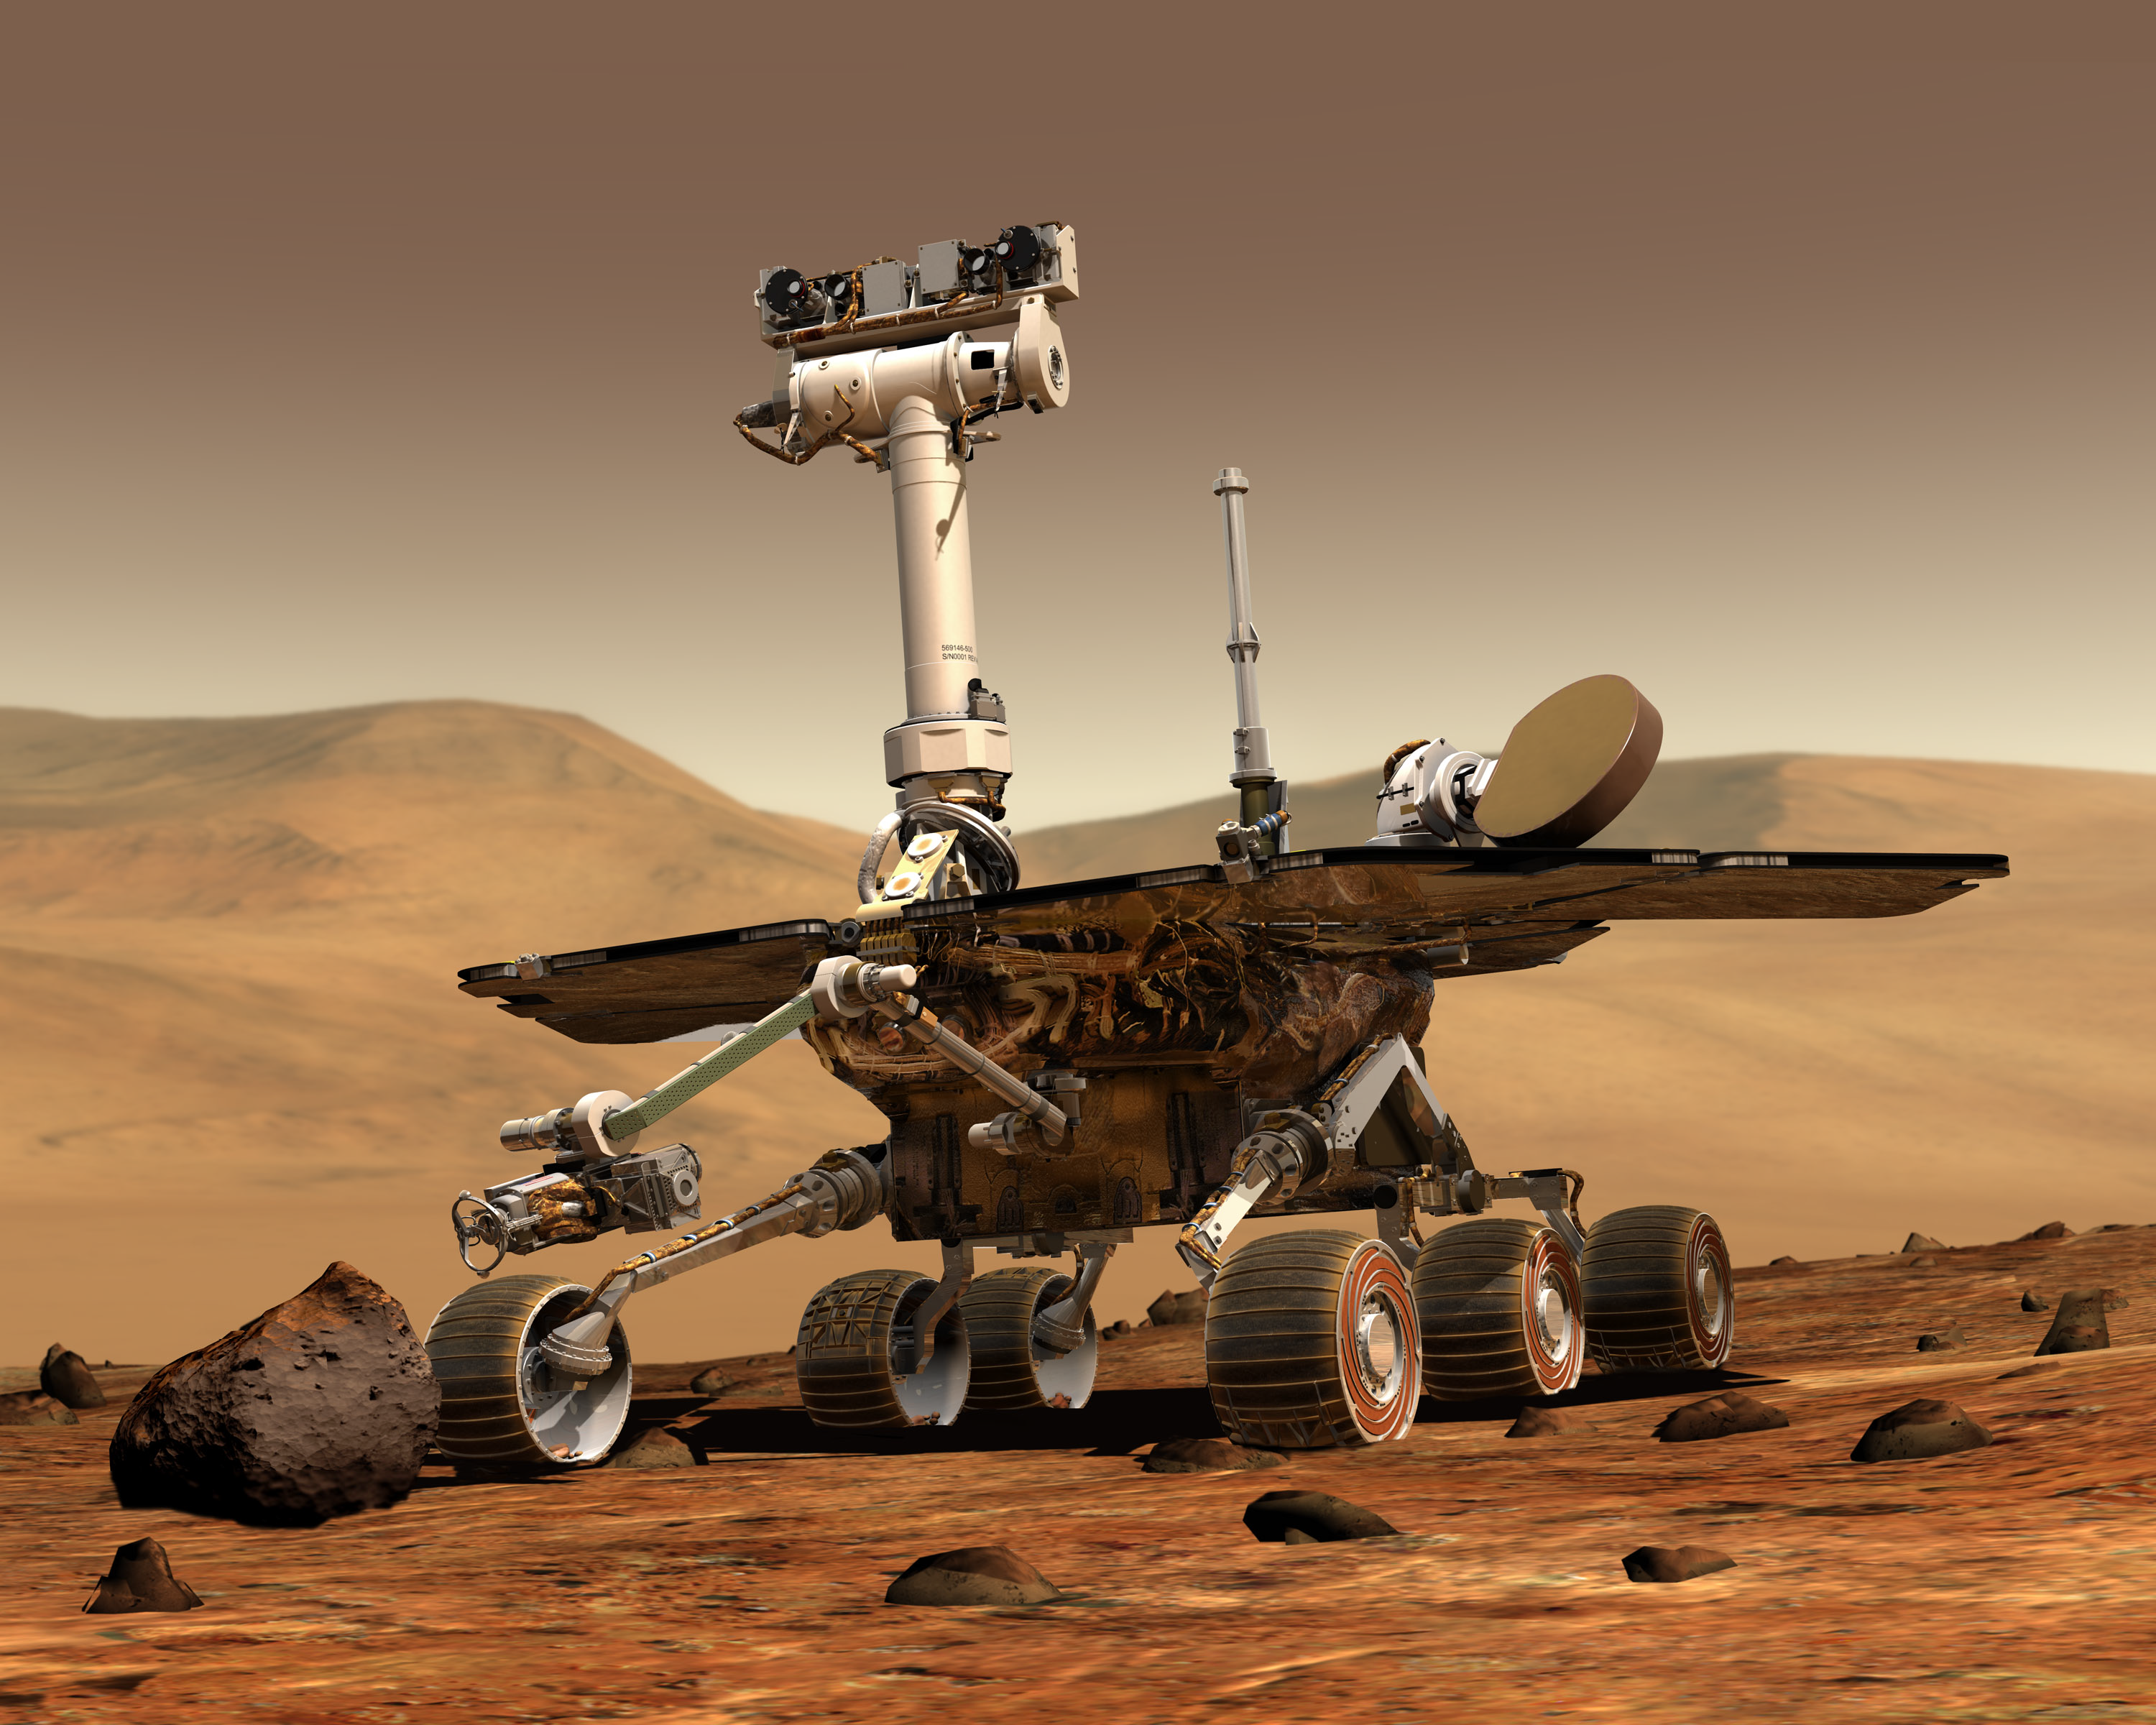
\includegraphics[width=.95\textwidth]{images/fig_01}
\end{center}
\end{minipage}

\begin{minipage}[c]{.47\linewidth}
\begin{center}
\includegraphics[height=5cm]{images/fig_02_bis}
\end{center}
\end{minipage}
\hfill
\begin{minipage}[c]{.47\linewidth}
\begin{center}
\includegraphics[height=5cm]{images/fig_03_bis}
\end{center}
\end{minipage}

C’est une équation différentielle linéaire du premier ordre dont la solution analytique est connue, ce qui permet de comparer la solution approchée à la solution exacte :
\begin{itemize}
\item au démarrage : $\omega(t)=\omega_c\left(1-e^{-\dfrac{t}{\tau}}\right)$;
\item à l'arrêt : $\omega(t)=\omega_c e^{-\dfrac{t}{\tau}}$.
\end{itemize}

\subsection{Méthode d'Euler explicite}
\begin{resultat}
La relation de récurrence s’écrit : $y_{k+1}=y_k+hf(y_k,t_k)$
\end{resultat}

Appliquons cette méthode à notre cas d'étude de cas :
$$\omega_{k+1}=\omega_k+h \dfrac{\omega_c-\omega_k}{\tau}$$

D’où :
$$
\omega_{k+1}=\omega_k \left(1-\dfrac{h}{\tau}\right)+\omega_c \dfrac{h}{\tau}
\quad \quad \quad 
\omega_k=\omega_0 \left(1-\dfrac{h}{\tau}\right)^k+\omega_c\left(1-\left(1-\dfrac{h}{\tau}\right)^k \right)
$$
Pour seulement 20 points, regardons ce que donne la méthode d’Euler explicite.

\begin{minipage}[c]{.47\linewidth}
\begin{center}
\includegraphics[width=.95\textwidth]{images/fig_04_bis}
\end{center}
\end{minipage}
\hfill
\begin{minipage}[c]{.47\linewidth}
\begin{center}
\includegraphics[width=.95\textwidth]{images/fig_05_bis}
\end{center}
\end{minipage}

\begin{exemple}
Donner la (ou les) fonctions python permettant de calculer un tableau contenant les $n$ couples $[\text{temps}_i,\omega_i]$. 
\vspace{10cm}
\end{exemple}

\subsubsection{Rapidité}
La rapidité de la méthode d’Euler explicite ne dépend que des opérations de l’équation de récurrence et du nombre d’itérations souhaitées $n$. Ainsi, nous aurons un temps de calcul directement proportionnel au facteur $n$ (et donc une complexité $\mathcal{O}(n)$).
\subsubsection{Précison -- Calcul d'erreur}

\begin{center}
\includegraphics[width=.8\textwidth]{images/fig_06}
\end{center}

Cherchons l’erreur commise par la méthode d’Euler :
$$e_{k+1}=|y(t_{k+1} )-y_{k+1} |<|y(t_{k+1} )-\tilde{y}_{k+1} |+|\tilde{y}_{k+1}-y_{k+1} |$$
$$e_{k+1}<e_{k+1}^{\text{loc}}+e_{k+1}^{\text{cumu}}$$

\paragraph{Calcul de de l’erreur locale (ou erreur de consistance)}
$$e_{k+1}^{\text{loc}}=|y(t_{k+1} )-\tilde{y}_{k+1} |=|y(t_{k+1} )-y(t_k )-hf(y(t_k ),t_k ) |$$

Avec le développement de Taylor au deuxième ordre, on obtient :

$$e_{k+1}^{\text{loc}}=|y(t_{k+1} )-\tilde{y}_{k+1} |=\left|y(t_{k+1} )-y(t_k )-h \dfrac{dy(t)}{dt}\right|=\left|\dfrac{h^2}{2}  \dfrac{d^2y(t)}{dt^2} +o(h^2 ) \right|$$


$$
e_{k+1}^{\text{loc}}<Kh^2
$$

Pour le moteur, l’erreur locale peut être majorée par :
$$e_{k+1}^{\text{loc}}=|\omega(t_{k+1} )-\tilde{\omega}_{k+1} |=\left|\dfrac{h^2}{2}  \dfrac{d^2 \omega}{dt^2}+o(h^2 ) \right|<Kh^2$$
$$e_{k+1}^{\text{loc}}=\left| \dfrac{h^2}{2\tau^2 } (\omega-\omega_c)+o(h^2 ) \right|<\dfrac{\omega_c}{2\tau^2 } h^2$$

\paragraph{Calcul de l’erreur cumulée}

$$e_{k+1}^{\text{cumu}}=|\tilde{y}_{k+1}-y_{k+1} |=|y(t_k )+hf(y(t_k ),t_k )-y_k-hf(y_k,t_k ) |$$
$$e_{k+1}^{\text{cumu}}<|y(t_k )-y_k |+h|f(y(t_k ),t_k )-f(y_k,t_k ) |$$

Or f est une fonction L-Lipschitzienne, c’est-à-dire pour tout $y_1$, $y_2$ et $t$ on a l’inéquation :
$$|f(y_2,t)-f(y_1,t) |\leq L|y_2-y_1 |$$
On en déduit l’expression de l’erreur cumulée en fonction de l’erreur du rang précédent :
$$e_{k+1}^{\text{cumu}}<(1+hL)|y(t_k )-y_k |$$


Pour le moteur, la constante de Lipschitz est :
$$
|f(\omega_{c_2},t)-f(\omega_{c_1},t) |
= \left|\dfrac{\omega_c-\omega_{c_2}}{\tau}-\dfrac{\omega_c-\omega_{c_1}}{\tau}\right|
\leq \dfrac{1}{\tau} |\omega_{c_2}-\omega_{c_1} |
$$
$$e_{k+1}^{\text{cumu}}<(1+h/\tau)|\omega_c(t_k )-\omega_{c_k} |=(1+h/\tau) e_k$$

\paragraph{Calcul de l’erreur globale}
$$e_{k+1}<e_{k+1}^{\text{loc}}+e_{k+1}^{\text{cumu}}$$
$$e_{k+1}<Kh^2+|1+hL| e_k<Kh^2  (|1+hL|^k-1)/hL+|1+hL|^k e_0$$
$$e_k<Kh (e^{(T_1-T_0 )L}-1)/L+|y(T_0 )-y_0 | e^{(T_1-T_0 )L}$$
Pour le cas du moteur, l’erreur est donc majorée.Si l’on considère que la valeur initiale est exacte, nous avons :
$$e_k<\dfrac{\omega_c}{2}  \dfrac{h}{\tau} \left(e^{\dfrac{T}{\tau}}-1\right)= \dfrac{\omega_c}{2}  \dfrac{T}{n\tau} \left(e^{\dfrac{T}{\tau}}-1\right)$$
L’erreur est donc majorée par un terme proportionnelle à 1/n ce qui montre que plus n sera grand plus l’erreur sera petite. Étant donné que nous connaissons la valeur exacte, il est possible de calculer plus précisément l’erreur.
$$e_k=\left|\omega(t_k)-\omega_k \right|=\omega_c\left|e^{-\dfrac{t_k}{\tau}}-\left(1-\dfrac{h}{\tau}\right)^k \right|<\dfrac{\omega_c}{2n}  \dfrac{T^2}{\tau^2}  e^{-\dfrac{t_k}{\tau}}$$

Pour notre exemple l’erreur maximale est de 62 rad/s en $t=\tau$ si l’on prend n=10.
\paragraph{Influence du pas de temps $h=T/n$ sur la précision}

\begin{center}
\includegraphics[width=.8\textwidth]{images/fig_07_bis}
\end{center}

On remarque dans cet exemple que l’erreur diminue avec l’augmentation du pas et que le schéma explicite donne une approximation plus grande que la réalité, pour le cas du démarrage (et plus petite dans le cas de l’arrêt du moteur).


\subsubsection{Stabilité -- Influence du paramètre $\dfrac{h}{\tau}$}

\begin{center}
\includegraphics[width=.8\textwidth]{images/fig_08_bis}
\end{center}

On remarque que le pas de temps $h$ doit être en adéquation avec la constante de temps $\tau$. Pour la valeur de 0,07, le schéma d’intégration oscille autour de la solution exacte et pour une valeur de 0,05 le schéma n’est pas stable :
$$\omega_k=\omega_c\left[1-(1-\dfrac{h}{\tau})^k \right]=\omega_c[(1-(-1))^k ]=2\text{ ou }\omega_c \text{ pour } \tau=\dfrac{h}{2}=0,05 $$

Au-delà de  cette valeur la suite diverge.

En conclusion, le pas de temps d’un schéma explicite doit être choisi suffisamment petit devant les constantes de temps de l’équation différentielle pour éviter des instabilités numériques.

\subsection{Méthode d'Euler implicite}
La relation de récurrence s’écrit : 
$$y_{k+1}=y_k+hf(y_{k+1},t_k)$$

Appliquons cette méthode à notre étude de cas :
$$\omega_{c_{k+1}}=\omega_{c_k}+h (\omega_c-\omega_{c_{k+1}})/\tau$$

Il faut donc résoudre une équation afin de déterminer $\omega_{c_{k+1}}$. Dans notre étude de cas, la résolution est aisée et on obtient :
$$\omega_{c_{k+1}}=\omega_{c_k}  1/(1+h⁄\tau)+\omega_c (h⁄\tau)/(1+h⁄\tau)$$

D’où :


\begin{minipage}[c]{.47\linewidth}
\begin{center}
\includegraphics[width=.95\textwidth]{images/fig_09}
\end{center}
\end{minipage}
\hfill
\begin{minipage}[c]{.47\linewidth}
\begin{center}
\includegraphics[width=.95\textwidth]{images/fig_10}
\end{center}
\end{minipage}

\subsubsection{Rapidité}

Ici, on remarque tout de suite qu’il faut résoudre une équation non linéaire du type (voir cours précédent):
$g(y_{k+1},y_k)=0$.

La rapidité dépendra donc de la méthode numérique de résolution de cette équation à chaque itération. Dans le cas où cette équation est particulièrement longue à résoudre, alors la méthode implicite est beaucoup plus lente que la méthode explicite.

Dans notre cas, la résolution n’est pas faite par la machine ; la rapidité sera donc du même ordre de grandeur que celle du schéma explicite.


\subsubsection{Précison -- Calcul d'erreur}

Le calcul de la précision ne change pas et la majoration de l’erreur reste :
$$e_k<Kh (e^{(T_1-T_0 )L}-1)/L+|y(T_0 )-y_0 | e^{(T_1-T_0 )L}$$
Pour le cas du moteur, l’erreur est donc majorée, si l’on considère que la valeur initiale est exacte, par :
$$e_k<\omega_c/2  h/\tau (e^(T/\tau)-1)=\omega_c/2  T/n\tau (e^(T/\tau)-1)$$

Pour notre exemple l’erreur maximale est de 41 rad/s en $t=\tau$ si l’on prend n=10. L’erreur maximale est plus faible que celle du schéma explicite.


\begin{center}
\includegraphics[width=.8\textwidth]{images/fig_11}
\end{center}

On note ici que le schéma implicite donne toujours une valeur plus petite que la valeur exacte dans le cas du démarrage.

\subsubsection{Stabilité -- Influence du paramètre $\dfrac{h}{\tau}$}

\begin{center}
\includegraphics[width=.8\textwidth]{images/fig_12}
\end{center}

Seule la constante de temps change, sur le graphique,on remarque que le schéma n’oscille pas autour de la solution exacte malgré $h>\tau$.

$$ 
\omega_c{_{k+1}}=(\omega_{c_k}+\omega_c h⁄\tau)/(1+h⁄\tau)=\omega_{c_0}/(1+h⁄\tau)^(k+1) +\omega_c (h⁄\tau)/(1+h⁄\tau)  (1-(1/(1+h⁄\tau))^(k+1))/(1-1/(1+h⁄\tau))$$

$$\omega_{c_k}=\omega_{c_0}/(1+h⁄\tau)^k +\omega_c[1-(1/(1+h⁄\tau))^k ]$$
La suite $\omega_{c_k}$ converge quelques soit le pas de temps h choisi.Par contre, plus la constante de temps $\tau$ diminue, moins le schéma est précis. En effet, l’augmentation de la raideur (forte variation de la dérivée) engendre des erreurs importantes.
En conclusion, le schéma implicite est beaucoup plus stable que le schéma explicite au détriment de la rapidité (résolution numérique d’une équation).

\section{Réduction de l'ordre d'une équation différentielle}


\begin{minipage}[c]{.25\linewidth}
\begin{center}
\includegraphics[width=.95\textwidth]{images/fig_13}
\end{center}
\end{minipage}
\hfill
\begin{minipage}[c]{.7\linewidth}
Nous avons vu que le problème de Cauchy peut être généralisé à plusieurs dimensions. A partir de ce constat, il est possible de transposer, tous les systèmes d’équations différentielles en un problème de Cauchy généralisé. L’idée est donc de réduire l’ordre de l’équation différentielle en augmentant la dimension du problème.
Pour illustrer ce propos prenons les équations dynamiques du régulateur de Watt :
L’équation de dynamique peut s’écrire :

$$(J+m_c a^2  \sin^2 \theta ) \ddot{\theta}+\dfrac{1}{2} (m_c a^2 \dot{\theta}^2+m_b L^2 \omega_c^2 ) \sin 2\theta +C(t)=0$$

Où $J$ est un moment d’inertie, $a$ une longueur caractéristique et $C$ un couple.
\end{minipage}



Cette équation dynamique est non linéaire, elle peut s’écrire sous la forme : $\ddot{\theta}=f(\dot{\theta},\theta,t)$. Posons alors le vecteur d’état $\vect{Y}$ tel que $\vect{Y}=\left(\begin{array}{c} \dot{\theta}\\ \theta \end{array}\right) =\left(\begin{array}{c} y_1 \\ y_2 \end{array}\right)$. 
Le système d’équation devient alors :
$$
\left\{\begin{array}{l}
\dfrac{d\theta}{dt} = \dot{\theta} \\
\dfrac{d\dot{\theta}}{dt} = - \dfrac{((m_c a^2 \dot{\theta}^2+m_b L^2 \omega^2 ) \sin 2\theta +C(t)}{2(J+m_c a^2  \sin^2\theta}
\end{array}\right.
$$

$$
\left\{\begin{array}{l}
\dfrac{dy_2}{dt} = y_1 \\
\dfrac{dy_1}{dt} = - \dfrac{((m_c a^2 y_1^2+m_b L^2 \omega^2 ) \sin 2 y_2 +C(t)}{2(J+m_c a^2  \sin^2y_2}
\end{array}\right.
\quad
\Longrightarrow
\quad
\dfrac{d\vect{Y}}{dt} = \vect{F}\left(\vect{Y},t\right)
$$


En conclusion, les équations différentielles d’ordre $n$ se ramènent à un système d’équations différentielles d’ordre 1 dont la variable est un vecteur caractérisant l’état du système. En automatique, ce type de méthode est souvent utilisé et est appelé la représentation d’état.


\begin{thebibliography}{2}
\bibitem{1}{Sylvie Delabriere, Équations différentielles, méthodes de résolution numérique -- Approximation numérique des fonctions, des intégrales, des solutions d'équations. Équations différentielles : approximation numérique des solutions.}
\bibitem{2}{Wack et Al., L’informatique pour tous en classes préparatoires aux grandes écoles, Editions Eyrolles.}
\bibitem{3}{Olivier Guindet, Résolution d'un problème dynamique par la méthode d'Euler, UPSTI.}
\bibitem{4}{Alain Caignot, Marc Derumaux, Résolution des équations différentielles, UPSTI.}
%\bibitem{1}{Adrien Petri, \textit{Analyse numérique : Intégration numérique}, Notes de cours de TSI 1, Lycée Rouvière, Toulon.}
\end{thebibliography}
\end{document}


